\documentclass[1p]{elsarticle_modified}
%\bibliographystyle{elsarticle-num}

%\usepackage[colorlinks]{hyperref}
%\usepackage{abbrmath_seonhwa} %\Abb, \Ascr, \Acal ,\Abf, \Afrak
\usepackage{amsfonts}
\usepackage{amssymb}
\usepackage{amsmath}
\usepackage{amsthm}
\usepackage{scalefnt}
\usepackage{amsbsy}
\usepackage{kotex}
\usepackage{caption}
\usepackage{subfig}
\usepackage{color}
\usepackage{graphicx}
\usepackage{xcolor} %% white, black, red, green, blue, cyan, magenta, yellow
\usepackage{float}
\usepackage{setspace}
\usepackage{hyperref}

\usepackage{tikz}
\usetikzlibrary{arrows}

\usepackage{multirow}
\usepackage{array} % fixed length table
\usepackage{hhline}

%%%%%%%%%%%%%%%%%%%%%
\makeatletter
\renewcommand*\env@matrix[1][\arraystretch]{%
	\edef\arraystretch{#1}%
	\hskip -\arraycolsep
	\let\@ifnextchar\new@ifnextchar
	\array{*\c@MaxMatrixCols c}}
\makeatother %https://tex.stackexchange.com/questions/14071/how-can-i-increase-the-line-spacing-in-a-matrix
%%%%%%%%%%%%%%%

\usepackage[normalem]{ulem}

\newcommand{\msout}[1]{\ifmmode\text{\sout{\ensuremath{#1}}}\else\sout{#1}\fi}
%SOURCE: \msout is \stkout macro in https://tex.stackexchange.com/questions/20609/strikeout-in-math-mode

\newcommand{\cancel}[1]{
	\ifmmode
	{\color{red}\msout{#1}}
	\else
	{\color{red}\sout{#1}}
	\fi
}

\newcommand{\add}[1]{
	{\color{blue}\uwave{#1}}
}

\newcommand{\replace}[2]{
	\ifmmode
	{\color{red}\msout{#1}}{\color{blue}\uwave{#2}}
	\else
	{\color{red}\sout{#1}}{\color{blue}\uwave{#2}}
	\fi
}

\newcommand{\Sol}{\mathcal{S}} %segment
\newcommand{\D}{D} %diagram
\newcommand{\A}{\mathcal{A}} %arc


%%%%%%%%%%%%%%%%%%%%%%%%%%%%%5 test

\def\sl{\operatorname{\textup{SL}}(2,\Cbb)}
\def\psl{\operatorname{\textup{PSL}}(2,\Cbb)}
\def\quan{\mkern 1mu \triangleright \mkern 1mu}

\theoremstyle{definition}
\newtheorem{thm}{Theorem}[section]
\newtheorem{prop}[thm]{Proposition}
\newtheorem{lem}[thm]{Lemma}
\newtheorem{ques}[thm]{Question}
\newtheorem{cor}[thm]{Corollary}
\newtheorem{defn}[thm]{Definition}
\newtheorem{exam}[thm]{Example}
\newtheorem{rmk}[thm]{Remark}
\newtheorem{alg}[thm]{Algorithm}

\newcommand{\I}{\sqrt{-1}}
\begin{document}

%\begin{frontmatter}
%
%\title{Boundary parabolic representations of knots up to 8 crossings}
%
%%% Group authors per affiliation:
%\author{Yunhi Cho} 
%\address{Department of Mathematics, University of Seoul, Seoul, Korea}
%\ead{yhcho@uos.ac.kr}
%
%
%\author{Seonhwa Kim} %\fnref{s_kim}}
%\address{Center for Geometry and Physics, Institute for Basic Science, Pohang, 37673, Korea}
%\ead{ryeona17@ibs.re.kr}
%
%\author{Hyuk Kim}
%\address{Department of Mathematical Sciences, Seoul National University, Seoul 08826, Korea}
%\ead{hyukkim@snu.ac.kr}
%
%\author{Seokbeom Yoon}
%\address{Department of Mathematical Sciences, Seoul National University, Seoul, 08826,  Korea}
%\ead{sbyoon15@snu.ac.kr}
%
%\begin{abstract}
%We find all boundary parabolic representation of knots up to 8 crossings.
%
%\end{abstract}
%\begin{keyword}
%    \MSC[2010] 57M25 
%\end{keyword}
%
%\end{frontmatter}

%\linenumbers
%\tableofcontents
%
\newcommand\colored[1]{\textcolor{white}{\rule[-0.35ex]{0.8em}{1.4ex}}\kern-0.8em\color{red} #1}%
%\newcommand\colored[1]{\textcolor{white}{ #1}\kern-2.17ex	\textcolor{white}{ #1}\kern-1.81ex	\textcolor{white}{ #1}\kern-2.15ex\color{red}#1	}

{\Large $\underline{12n_{0638}~(K12n_{0638})}$}

\setlength{\tabcolsep}{10pt}
\renewcommand{\arraystretch}{1.6}
\vspace{1cm}\begin{tabular}{m{100pt}>{\centering\arraybackslash}m{274pt}}
\multirow{5}{120pt}{
	\centering
	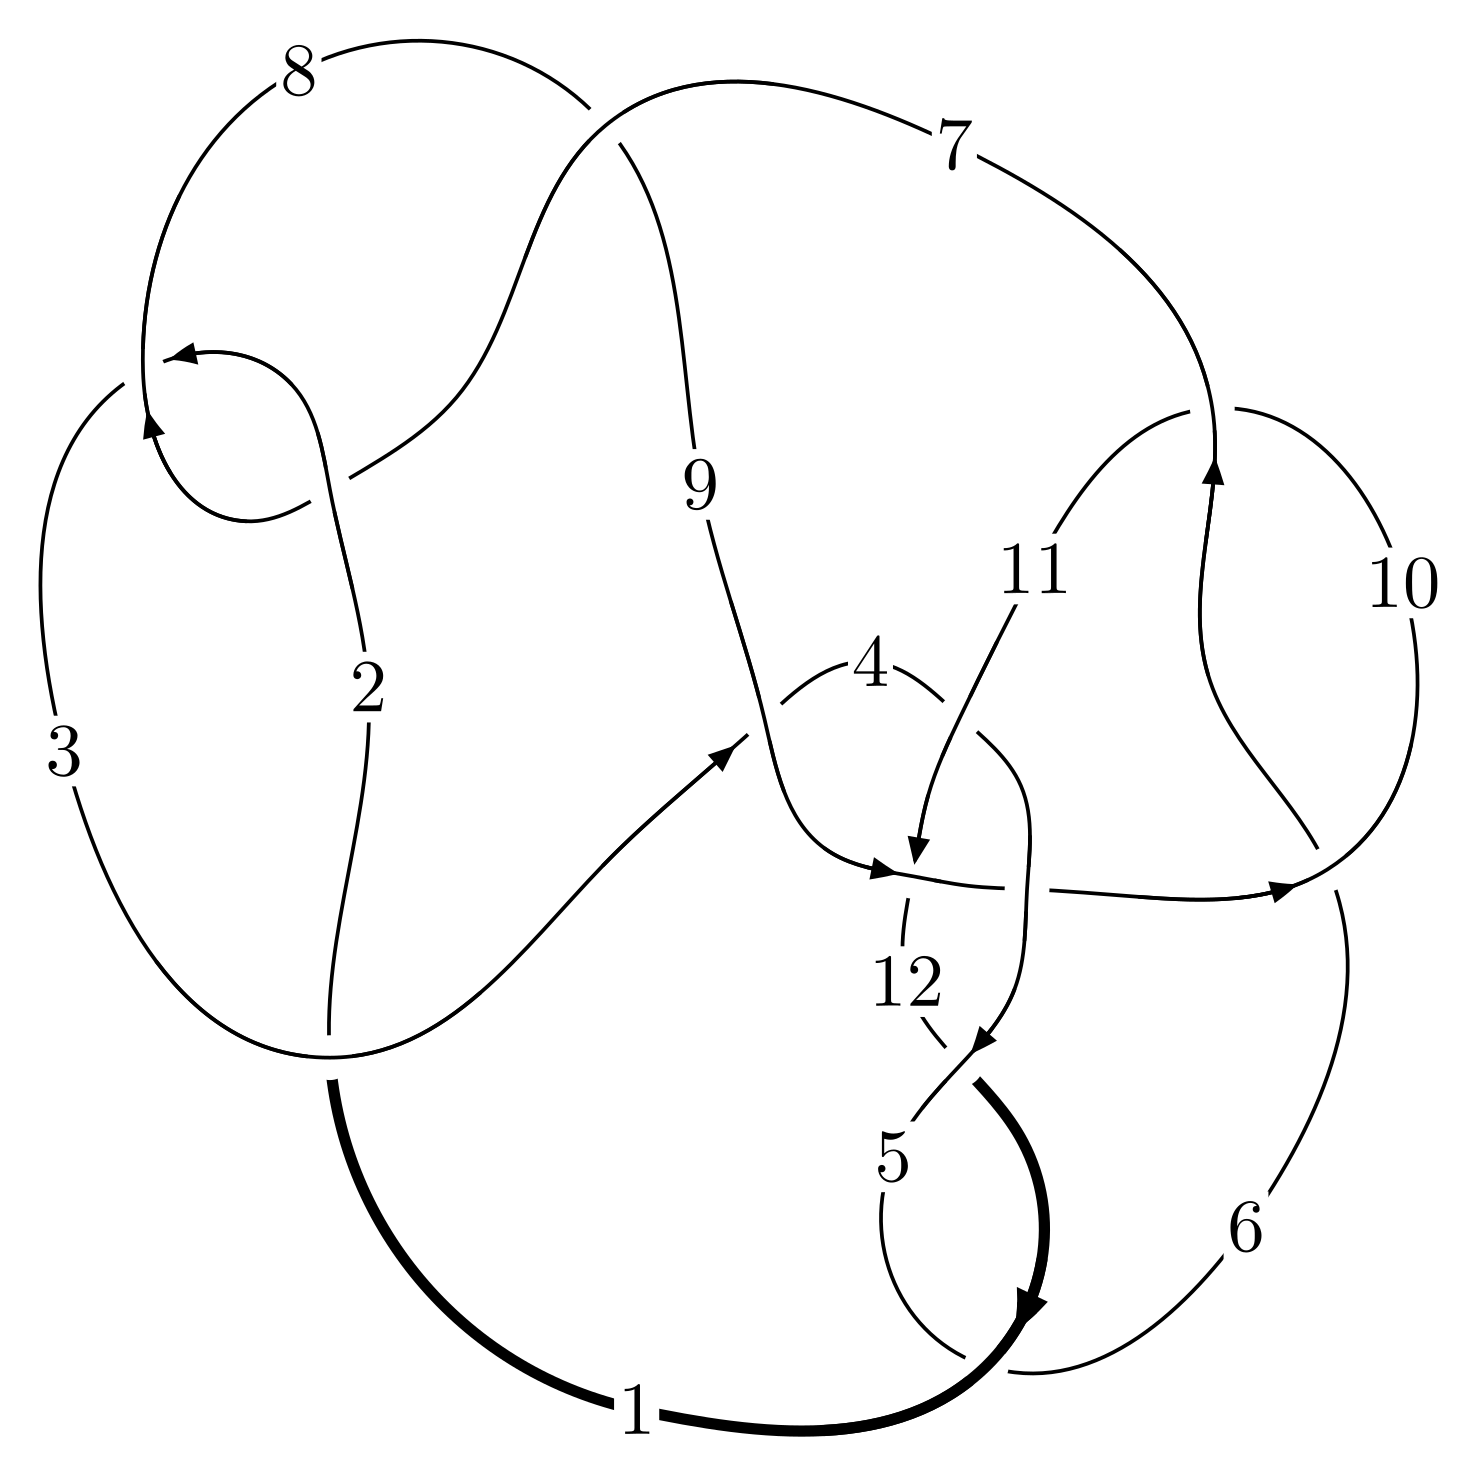
\includegraphics[width=112pt]{../../../GIT/diagram.site/Diagrams/png/2727_12n_0638.png}\\
\ \ \ A knot diagram\footnotemark}&
\allowdisplaybreaks
\textbf{Linearized knot diagam} \\
\cline{2-2}
 &
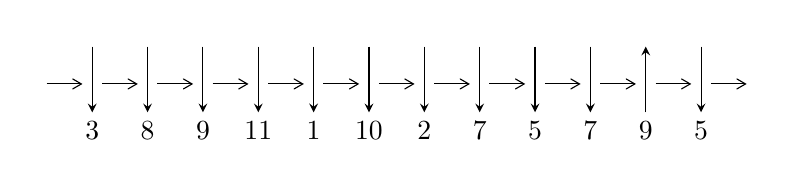
\begin{tikzpicture}[x=20pt, y=17pt]
	% nodes
	\node (C0) at (0, 0) {};
	\node (C1) at (1, 0) {};
	\node (C1U) at (1, +1) {};
	\node (C1D) at (1, -1) {3};

	\node (C2) at (2, 0) {};
	\node (C2U) at (2, +1) {};
	\node (C2D) at (2, -1) {8};

	\node (C3) at (3, 0) {};
	\node (C3U) at (3, +1) {};
	\node (C3D) at (3, -1) {9};

	\node (C4) at (4, 0) {};
	\node (C4U) at (4, +1) {};
	\node (C4D) at (4, -1) {11};

	\node (C5) at (5, 0) {};
	\node (C5U) at (5, +1) {};
	\node (C5D) at (5, -1) {1};

	\node (C6) at (6, 0) {};
	\node (C6U) at (6, +1) {};
	\node (C6D) at (6, -1) {10};

	\node (C7) at (7, 0) {};
	\node (C7U) at (7, +1) {};
	\node (C7D) at (7, -1) {2};

	\node (C8) at (8, 0) {};
	\node (C8U) at (8, +1) {};
	\node (C8D) at (8, -1) {7};

	\node (C9) at (9, 0) {};
	\node (C9U) at (9, +1) {};
	\node (C9D) at (9, -1) {5};

	\node (C10) at (10, 0) {};
	\node (C10U) at (10, +1) {};
	\node (C10D) at (10, -1) {7};

	\node (C11) at (11, 0) {};
	\node (C11U) at (11, +1) {};
	\node (C11D) at (11, -1) {9};

	\node (C12) at (12, 0) {};
	\node (C12U) at (12, +1) {};
	\node (C12D) at (12, -1) {5};
	\node (C13) at (13, 0) {};

	% arrows
	\draw[->,>={angle 60}]
	(C0) edge (C1) (C1) edge (C2) (C2) edge (C3) (C3) edge (C4) (C4) edge (C5) (C5) edge (C6) (C6) edge (C7) (C7) edge (C8) (C8) edge (C9) (C9) edge (C10) (C10) edge (C11) (C11) edge (C12) (C12) edge (C13) ;	\draw[->,>=stealth]
	(C1U) edge (C1D) (C2U) edge (C2D) (C3U) edge (C3D) (C4U) edge (C4D) (C5U) edge (C5D) (C6U) edge (C6D) (C7U) edge (C7D) (C8U) edge (C8D) (C9U) edge (C9D) (C10U) edge (C10D) (C11D) edge (C11U) (C12U) edge (C12D) ;
	\end{tikzpicture} \\
\hhline{~~} \\& 
\textbf{Solving Sequence} \\ \cline{2-2} 
 &
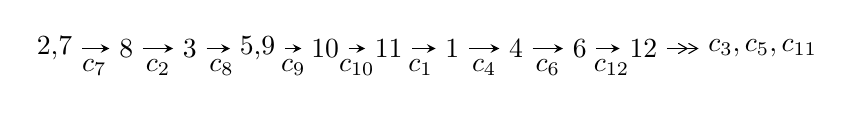
\begin{tikzpicture}[x=23pt, y=7pt]
	% node
	\node (A0) at (-1/8, 0) {2,7};
	\node (A1) at (1, 0) {8};
	\node (A2) at (2, 0) {3};
	\node (A3) at (49/16, 0) {5,9};
	\node (A4) at (33/8, 0) {10};
	\node (A5) at (41/8, 0) {11};
	\node (A6) at (49/8, 0) {1};
	\node (A7) at (57/8, 0) {4};
	\node (A8) at (65/8, 0) {6};
	\node (A9) at (73/8, 0) {12};
	\node (C1) at (1/2, -1) {$c_{7}$};
	\node (C2) at (3/2, -1) {$c_{2}$};
	\node (C3) at (5/2, -1) {$c_{8}$};
	\node (C4) at (29/8, -1) {$c_{9}$};
	\node (C5) at (37/8, -1) {$c_{10}$};
	\node (C6) at (45/8, -1) {$c_{1}$};
	\node (C7) at (53/8, -1) {$c_{4}$};
	\node (C8) at (61/8, -1) {$c_{6}$};
	\node (C9) at (69/8, -1) {$c_{12}$};
	\node (A10) at (11, 0) {$c_{3},c_{5},c_{11}$};

	% edge
	\draw[->,>=stealth]	
	(A0) edge (A1) (A1) edge (A2) (A2) edge (A3) (A3) edge (A4) (A4) edge (A5) (A5) edge (A6) (A6) edge (A7) (A7) edge (A8) (A8) edge (A9) ;
	\draw[->>,>={angle 60}]	
	(A9) edge (A10);
\end{tikzpicture} \\ 

\end{tabular} \\

\footnotetext{
The image of knot diagram is generated by the software ``\textbf{Draw programme}" developed by Andrew Bartholomew(\url{http://www.layer8.co.uk/maths/draw/index.htm\#Running-draw}), where we modified some parts for our purpose(\url{https://github.com/CATsTAILs/LinksPainter}).
}\phantom \\ \newline 
\centering \textbf{Ideals for irreducible components\footnotemark of $X_{\text{par}}$} 
 
\begin{align*}
I^u_{1}&=\langle 
- u^{14}-3 u^{13}+\cdots+2 b-2,\;7 u^{14}+29 u^{13}+\cdots+4 a+24,\;u^{15}+5 u^{14}+\cdots+18 u+4\rangle \\
I^u_{2}&=\langle 
u^{10}+u^9- u^8+4 u^6+3 u^5-2 u^4+3 u^2+b+2 u,\;u^{10}+3 u^6+u^5+u^4- u^3+2 u^2+a+2 u+1,\\
\phantom{I^u_{2}}&\phantom{= \langle  }u^{11}+u^{10}- u^9- u^8+4 u^7+4 u^6-2 u^5-3 u^4+3 u^3+4 u^2-1\rangle \\
I^u_{3}&=\langle 
b+2,\;a+1,\;u-1\rangle \\
I^u_{4}&=\langle 
a^3+2 a^2+3 b+a+5,\;a^4+a^3+2 a^2+4 a+1,\;u-1\rangle \\
\\
\end{align*}
\raggedright * 4 irreducible components of $\dim_{\mathbb{C}}=0$, with total 31 representations.\\
\footnotetext{All coefficients of polynomials are rational numbers. But the coefficients are sometimes approximated in decimal forms when there is not enough margin.}
\newpage
\renewcommand{\arraystretch}{1}
\centering \section*{I. $I^u_{1}= \langle - u^{14}-3 u^{13}+\cdots+2 b-2,\;7 u^{14}+29 u^{13}+\cdots+4 a+24,\;u^{15}+5 u^{14}+\cdots+18 u+4 \rangle$}
\flushleft \textbf{(i) Arc colorings}\\
\begin{tabular}{m{7pt} m{180pt} m{7pt} m{180pt} }
\flushright $a_{2}=$&$\begin{pmatrix}0\\u\end{pmatrix}$ \\
\flushright $a_{7}=$&$\begin{pmatrix}1\\0\end{pmatrix}$ \\
\flushright $a_{8}=$&$\begin{pmatrix}1\\u^2\end{pmatrix}$ \\
\flushright $a_{3}=$&$\begin{pmatrix}- u\\- u^3+u\end{pmatrix}$ \\
\flushright $a_{5}=$&$\begin{pmatrix}-\frac{7}{4} u^{14}-\frac{29}{4} u^{13}+\cdots-\frac{105}{4} u-6\\\frac{1}{2} u^{14}+\frac{3}{2} u^{13}+\cdots+\frac{11}{2} u+1\end{pmatrix}$ \\
\flushright $a_{9}=$&$\begin{pmatrix}- u^2+1\\u^2\end{pmatrix}$ \\
\flushright $a_{10}=$&$\begin{pmatrix}-\frac{1}{2} u^{14}-2 u^{13}+\cdots-\frac{9}{2} u-\frac{1}{2}\\\frac{1}{2} u^{14}+\frac{3}{2} u^{13}+\cdots+4 u^2+\frac{1}{2} u\end{pmatrix}$ \\
\flushright $a_{11}=$&$\begin{pmatrix}- u^{14}-\frac{7}{2} u^{13}+\cdots-5 u-\frac{1}{2}\\\frac{1}{2} u^{14}+\frac{3}{2} u^{13}+\cdots+4 u^2+\frac{1}{2} u\end{pmatrix}$ \\
\flushright $a_{1}=$&$\begin{pmatrix}u^3\\u^5- u^3+u\end{pmatrix}$ \\
\flushright $a_{4}=$&$\begin{pmatrix}u^7-2 u^5+2 u^3-2 u\\- u^7+u^5-2 u^3+u\end{pmatrix}$ \\
\flushright $a_{6}=$&$\begin{pmatrix}\frac{5}{4} u^{14}+\frac{23}{4} u^{13}+\cdots+\frac{79}{4} u+6\\-\frac{1}{2} u^{14}-\frac{3}{2} u^{13}+\cdots-\frac{9}{2} u-1\end{pmatrix}$ \\
\flushright $a_{12}=$&$\begin{pmatrix}-\frac{1}{2} u^{14}-2 u^{13}+\cdots-\frac{9}{2} u-\frac{3}{2}\\\frac{1}{2} u^{14}+\frac{3}{2} u^{13}+\cdots+3 u^2+\frac{3}{2} u\end{pmatrix}$\\&\end{tabular}
\flushleft \textbf{(ii) Obstruction class $= -1$}\\~\\
\flushleft \textbf{(iii) Cusp Shapes $= -9 u^{14}-39 u^{13}-62 u^{12}+12 u^{11}+189 u^{10}+271 u^9+58 u^8-259 u^7-277 u^6+33 u^5+223 u^4+70 u^3-138 u^2-142 u-54$}\\~\\
\newpage\renewcommand{\arraystretch}{1}
\flushleft \textbf{(iv) u-Polynomials at the component}\newline \\
\begin{tabular}{m{50pt}|m{274pt}}
Crossings & \hspace{64pt}u-Polynomials at each crossing \\
\hline $$\begin{aligned}c_{1},c_{8}\end{aligned}$$&$\begin{aligned}
&u^{15}+5 u^{14}+\cdots+108 u+16
\end{aligned}$\\
\hline $$\begin{aligned}c_{2},c_{7}\end{aligned}$$&$\begin{aligned}
&u^{15}+5 u^{14}+\cdots+18 u+4
\end{aligned}$\\
\hline $$\begin{aligned}c_{3}\end{aligned}$$&$\begin{aligned}
&u^{15}-7 u^{14}+\cdots-7974 u+2196
\end{aligned}$\\
\hline $$\begin{aligned}c_{4},c_{6},c_{10}\end{aligned}$$&$\begin{aligned}
&u^{15}-3 u^{14}+\cdots+2 u+1
\end{aligned}$\\
\hline $$\begin{aligned}c_{5},c_{9},c_{12}\end{aligned}$$&$\begin{aligned}
&u^{15}+2 u^{14}+\cdots-3 u-1
\end{aligned}$\\
\hline $$\begin{aligned}c_{11}\end{aligned}$$&$\begin{aligned}
&u^{15}+8 u^{14}+\cdots+26 u+2
\end{aligned}$\\
\hline
\end{tabular}\\~\\
\newpage\renewcommand{\arraystretch}{1}
\flushleft \textbf{(v) Riley Polynomials at the component}\newline \\
\begin{tabular}{m{50pt}|m{274pt}}
Crossings & \hspace{64pt}Riley Polynomials at each crossing \\
\hline $$\begin{aligned}c_{1},c_{8}\end{aligned}$$&$\begin{aligned}
&y^{15}+11 y^{14}+\cdots+4464 y-256
\end{aligned}$\\
\hline $$\begin{aligned}c_{2},c_{7}\end{aligned}$$&$\begin{aligned}
&y^{15}-5 y^{14}+\cdots+108 y-16
\end{aligned}$\\
\hline $$\begin{aligned}c_{3}\end{aligned}$$&$\begin{aligned}
&y^{15}-89 y^{14}+\cdots+102923820 y-4822416
\end{aligned}$\\
\hline $$\begin{aligned}c_{4},c_{6},c_{10}\end{aligned}$$&$\begin{aligned}
&y^{15}-41 y^{14}+\cdots+36 y-1
\end{aligned}$\\
\hline $$\begin{aligned}c_{5},c_{9},c_{12}\end{aligned}$$&$\begin{aligned}
&y^{15}-28 y^{14}+\cdots-11 y-1
\end{aligned}$\\
\hline $$\begin{aligned}c_{11}\end{aligned}$$&$\begin{aligned}
&y^{15}-38 y^{14}+\cdots+200 y-4
\end{aligned}$\\
\hline
\end{tabular}\\~\\
\newpage\flushleft \textbf{(vi) Complex Volumes and Cusp Shapes}
$$\begin{array}{c|c|c}  
\text{Solutions to }I^u_{1}& \I (\text{vol} + \sqrt{-1}CS) & \text{Cusp shape}\\
 \hline 
\begin{aligned}
u &= -0.606388 + 0.721644 I \\
a &= \phantom{-}1.39179 + 0.62558 I \\
b &= -0.960938 - 0.688802 I\end{aligned}
 & -0.178243 - 0.909766 I & -10.00645 + 2.94587 I \\ \hline\begin{aligned}
u &= -0.606388 - 0.721644 I \\
a &= \phantom{-}1.39179 - 0.62558 I \\
b &= -0.960938 + 0.688802 I\end{aligned}
 & -0.178243 + 0.909766 I & -10.00645 - 2.94587 I \\ \hline\begin{aligned}
u &= \phantom{-}1.08047\phantom{ +0.000000I} \\
a &= -0.675053\phantom{ +0.000000I} \\
b &= -1.51745\phantom{ +0.000000I}\end{aligned}
 & -5.54081\phantom{ +0.000000I} & -14.3560\phantom{ +0.000000I} \\ \hline\begin{aligned}
u &= \phantom{-}0.746431 + 0.514902 I \\
a &= \phantom{-}0.082980 - 0.242831 I \\
b &= \phantom{-}0.397865 - 0.145660 I\end{aligned}
 & \phantom{-}1.19505 - 1.99555 I & -7.66777 + 5.97030 I \\ \hline\begin{aligned}
u &= \phantom{-}0.746431 - 0.514902 I \\
a &= \phantom{-}0.082980 + 0.242831 I \\
b &= \phantom{-}0.397865 + 0.145660 I\end{aligned}
 & \phantom{-}1.19505 + 1.99555 I & -7.66777 - 5.97030 I \\ \hline\begin{aligned}
u &= -1.021710 + 0.661454 I \\
a &= -0.06650 - 1.96813 I \\
b &= -1.33073 + 0.86334 I\end{aligned}
 & -1.39940 + 6.23344 I & -10.94430 - 8.75401 I \\ \hline\begin{aligned}
u &= -1.021710 - 0.661454 I \\
a &= -0.06650 + 1.96813 I \\
b &= -1.33073 - 0.86334 I\end{aligned}
 & -1.39940 - 6.23344 I & -10.94430 + 8.75401 I \\ \hline\begin{aligned}
u &= -0.518806 + 1.107840 I \\
a &= -1.210170 - 0.046109 I \\
b &= \phantom{-}1.78546 + 0.11853 I\end{aligned}
 & -10.31580 - 3.71425 I & -10.43409 + 0.73580 I \\ \hline\begin{aligned}
u &= -0.518806 - 1.107840 I \\
a &= -1.210170 + 0.046109 I \\
b &= \phantom{-}1.78546 - 0.11853 I\end{aligned}
 & -10.31580 + 3.71425 I & -10.43409 - 0.73580 I \\ \hline\begin{aligned}
u &= -0.931933 + 0.895825 I \\
a &= -0.466639 + 0.398594 I \\
b &= \phantom{-}0.712541 + 0.015963 I\end{aligned}
 & \phantom{-}9.82516 + 3.30608 I & -14.5483 - 3.5573 I\\
 \hline 
 \end{array}$$\newpage$$\begin{array}{c|c|c}  
\text{Solutions to }I^u_{1}& \I (\text{vol} + \sqrt{-1}CS) & \text{Cusp shape}\\
 \hline 
\begin{aligned}
u &= -0.931933 - 0.895825 I \\
a &= -0.466639 - 0.398594 I \\
b &= \phantom{-}0.712541 - 0.015963 I\end{aligned}
 & \phantom{-}9.82516 - 3.30608 I & -14.5483 + 3.5573 I \\ \hline\begin{aligned}
u &= -1.21080 + 0.76031 I \\
a &= -0.31276 + 1.60256 I \\
b &= \phantom{-}1.83309 - 0.17932 I\end{aligned}
 & -12.5061 + 10.4262 I & -11.73103 - 4.47783 I \\ \hline\begin{aligned}
u &= -1.21080 - 0.76031 I \\
a &= -0.31276 - 1.60256 I \\
b &= \phantom{-}1.83309 + 0.17932 I\end{aligned}
 & -12.5061 - 10.4262 I & -11.73103 + 4.47783 I \\ \hline\begin{aligned}
u &= \phantom{-}1.46326\phantom{ +0.000000I} \\
a &= \phantom{-}0.512604\phantom{ +0.000000I} \\
b &= \phantom{-}1.84763\phantom{ +0.000000I}\end{aligned}
 & -18.0985\phantom{ +0.000000I} & -13.9500\phantom{ +0.000000I} \\ \hline\begin{aligned}
u &= -0.457334\phantom{ +0.000000I} \\
a &= \phantom{-}0.825053\phantom{ +0.000000I} \\
b &= -0.204761\phantom{ +0.000000I}\end{aligned}
 & -0.594889\phantom{ +0.000000I} & -17.0300\phantom{ +0.000000I}\\
 \hline 
 \end{array}$$\newpage\newpage\renewcommand{\arraystretch}{1}
\centering \section*{II. $I^u_{2}= \langle u^{10}+u^9- u^8+4 u^6+3 u^5-2 u^4+3 u^2+b+2 u,\;u^{10}+3 u^6+u^5+u^4- u^3+2 u^2+a+2 u+1,\;u^{11}+u^{10}+\cdots+4 u^2-1 \rangle$}
\flushleft \textbf{(i) Arc colorings}\\
\begin{tabular}{m{7pt} m{180pt} m{7pt} m{180pt} }
\flushright $a_{2}=$&$\begin{pmatrix}0\\u\end{pmatrix}$ \\
\flushright $a_{7}=$&$\begin{pmatrix}1\\0\end{pmatrix}$ \\
\flushright $a_{8}=$&$\begin{pmatrix}1\\u^2\end{pmatrix}$ \\
\flushright $a_{3}=$&$\begin{pmatrix}- u\\- u^3+u\end{pmatrix}$ \\
\flushright $a_{5}=$&$\begin{pmatrix}- u^{10}-3 u^6- u^5- u^4+u^3-2 u^2-2 u-1\\- u^{10}- u^9+u^8-4 u^6-3 u^5+2 u^4-3 u^2-2 u\end{pmatrix}$ \\
\flushright $a_{9}=$&$\begin{pmatrix}- u^2+1\\u^2\end{pmatrix}$ \\
\flushright $a_{10}=$&$\begin{pmatrix}- u^{10}+2 u^8-5 u^6+6 u^4-6 u^2- u+4\\u^{10}+u^9- u^8- u^7+4 u^6+3 u^5-2 u^4-2 u^3+3 u^2+2 u\end{pmatrix}$ \\
\flushright $a_{11}=$&$\begin{pmatrix}-2 u^{10}- u^9+3 u^8+u^7-9 u^6-3 u^5+8 u^4+2 u^3-9 u^2-3 u+4\\u^{10}+u^9- u^8- u^7+4 u^6+3 u^5-2 u^4-2 u^3+3 u^2+2 u\end{pmatrix}$ \\
\flushright $a_{1}=$&$\begin{pmatrix}u^3\\u^5- u^3+u\end{pmatrix}$ \\
\flushright $a_{4}=$&$\begin{pmatrix}u^7-2 u^5+2 u^3-2 u\\- u^7+u^5-2 u^3+u\end{pmatrix}$ \\
\flushright $a_{6}=$&$\begin{pmatrix}-2 u^{10}- u^9+u^8-7 u^6-3 u^5+u^4+u^3-5 u^2-3 u\\- u^{10}- u^9+u^8+u^7-4 u^6-4 u^5+2 u^4+2 u^3-3 u^2-3 u\end{pmatrix}$ \\
\flushright $a_{12}=$&$\begin{pmatrix}- u^{10}+2 u^8-5 u^6+6 u^4+u^3-5 u^2- u+3\\u^{10}+u^9- u^8- u^7+4 u^6+4 u^5-2 u^4-3 u^3+2 u^2+3 u\end{pmatrix}$\\&\end{tabular}
\flushleft \textbf{(ii) Obstruction class $= 1$}\\~\\
\flushleft \textbf{(iii) Cusp Shapes $= 2 u^{10}+2 u^7+8 u^6-2 u^5+u^3+10 u^2+u-10$}\\~\\
\newpage\renewcommand{\arraystretch}{1}
\flushleft \textbf{(iv) u-Polynomials at the component}\newline \\
\begin{tabular}{m{50pt}|m{274pt}}
Crossings & \hspace{64pt}u-Polynomials at each crossing \\
\hline $$\begin{aligned}c_{1}\end{aligned}$$&$\begin{aligned}
&u^{11}-3 u^{10}+\cdots+8 u-1
\end{aligned}$\\
\hline $$\begin{aligned}c_{2}\end{aligned}$$&$\begin{aligned}
&u^{11}- u^{10}- u^9+u^8+4 u^7-4 u^6-2 u^5+3 u^4+3 u^3-4 u^2+1
\end{aligned}$\\
\hline $$\begin{aligned}c_{3}\end{aligned}$$&$\begin{aligned}
&u^{11}- u^{10}+7 u^9+u^8-2 u^7+5 u^6+39 u^5-31 u^4+12 u^3- u^2-2 u+1
\end{aligned}$\\
\hline $$\begin{aligned}c_{4},c_{10}\end{aligned}$$&$\begin{aligned}
&u^{11}+2 u^{10}+2 u^9+2 u^8- u^7-3 u^6- u^5+2 u^3+3 u^2+u+1
\end{aligned}$\\
\hline $$\begin{aligned}c_{5},c_{9}\end{aligned}$$&$\begin{aligned}
&u^{11}+u^{10}+3 u^9+2 u^8- u^6-3 u^5- u^4+2 u^3+2 u^2+2 u+1
\end{aligned}$\\
\hline $$\begin{aligned}c_{6}\end{aligned}$$&$\begin{aligned}
&u^{11}-2 u^{10}+2 u^9-2 u^8- u^7+3 u^6- u^5+2 u^3-3 u^2+u-1
\end{aligned}$\\
\hline $$\begin{aligned}c_{7}\end{aligned}$$&$\begin{aligned}
&u^{11}+u^{10}- u^9- u^8+4 u^7+4 u^6-2 u^5-3 u^4+3 u^3+4 u^2-1
\end{aligned}$\\
\hline $$\begin{aligned}c_{8}\end{aligned}$$&$\begin{aligned}
&u^{11}+3 u^{10}+\cdots+8 u+1
\end{aligned}$\\
\hline $$\begin{aligned}c_{11}\end{aligned}$$&$\begin{aligned}
&u^{11}-11 u^{10}+\cdots-24 u+9
\end{aligned}$\\
\hline $$\begin{aligned}c_{12}\end{aligned}$$&$\begin{aligned}
&u^{11}- u^{10}+3 u^9-2 u^8+u^6-3 u^5+u^4+2 u^3-2 u^2+2 u-1
\end{aligned}$\\
\hline
\end{tabular}\\~\\
\newpage\renewcommand{\arraystretch}{1}
\flushleft \textbf{(v) Riley Polynomials at the component}\newline \\
\begin{tabular}{m{50pt}|m{274pt}}
Crossings & \hspace{64pt}Riley Polynomials at each crossing \\
\hline $$\begin{aligned}c_{1},c_{8}\end{aligned}$$&$\begin{aligned}
&y^{11}+13 y^{10}+\cdots+20 y-1
\end{aligned}$\\
\hline $$\begin{aligned}c_{2},c_{7}\end{aligned}$$&$\begin{aligned}
&y^{11}-3 y^{10}+\cdots+8 y-1
\end{aligned}$\\
\hline $$\begin{aligned}c_{3}\end{aligned}$$&$\begin{aligned}
&y^{11}+13 y^{10}+\cdots+6 y-1
\end{aligned}$\\
\hline $$\begin{aligned}c_{4},c_{6},c_{10}\end{aligned}$$&$\begin{aligned}
&y^{11}-6 y^9+2 y^8+13 y^7-9 y^6-15 y^5+8 y^4+8 y^3-5 y^2-5 y-1
\end{aligned}$\\
\hline $$\begin{aligned}c_{5},c_{9},c_{12}\end{aligned}$$&$\begin{aligned}
&y^{11}+5 y^{10}+5 y^9-8 y^8-8 y^7+15 y^6+9 y^5-13 y^4-2 y^3+6 y^2-1
\end{aligned}$\\
\hline $$\begin{aligned}c_{11}\end{aligned}$$&$\begin{aligned}
&y^{11}-23 y^{10}+\cdots-324 y-81
\end{aligned}$\\
\hline
\end{tabular}\\~\\
\newpage\flushleft \textbf{(vi) Complex Volumes and Cusp Shapes}
$$\begin{array}{c|c|c}  
\text{Solutions to }I^u_{2}& \I (\text{vol} + \sqrt{-1}CS) & \text{Cusp shape}\\
 \hline 
\begin{aligned}
u &= \phantom{-}0.859595 + 0.621070 I \\
a &= \phantom{-}0.264591 - 0.511619 I \\
b &= \phantom{-}1.184910 - 0.173635 I\end{aligned}
 & \phantom{-}5.06364 - 2.43633 I & -9.98510 + 2.91167 I \\ \hline\begin{aligned}
u &= \phantom{-}0.859595 - 0.621070 I \\
a &= \phantom{-}0.264591 + 0.511619 I \\
b &= \phantom{-}1.184910 + 0.173635 I\end{aligned}
 & \phantom{-}5.06364 + 2.43633 I & -9.98510 - 2.91167 I \\ \hline\begin{aligned}
u &= -0.715758 + 0.795244 I \\
a &= \phantom{-}1.83523 - 0.23082 I \\
b &= -1.61321 - 0.43685 I\end{aligned}
 & -1.149260 + 0.247570 I & -13.50982 - 0.73342 I \\ \hline\begin{aligned}
u &= -0.715758 - 0.795244 I \\
a &= \phantom{-}1.83523 + 0.23082 I \\
b &= -1.61321 + 0.43685 I\end{aligned}
 & -1.149260 - 0.247570 I & -13.50982 + 0.73342 I \\ \hline\begin{aligned}
u &= -0.791184 + 0.262463 I \\
a &= -0.50598 + 1.77609 I \\
b &= \phantom{-}0.389923 - 0.338442 I\end{aligned}
 & \phantom{-}3.12519 + 1.08690 I & -6.47529 - 6.28285 I \\ \hline\begin{aligned}
u &= -0.791184 - 0.262463 I \\
a &= -0.50598 - 1.77609 I \\
b &= \phantom{-}0.389923 + 0.338442 I\end{aligned}
 & \phantom{-}3.12519 - 1.08690 I & -6.47529 + 6.28285 I \\ \hline\begin{aligned}
u &= -1.006190 + 0.705559 I \\
a &= \phantom{-}0.60734 - 2.06814 I \\
b &= -1.77582 + 0.58284 I\end{aligned}
 & -2.06494 + 5.42980 I & -15.7370 - 3.3620 I \\ \hline\begin{aligned}
u &= -1.006190 - 0.705559 I \\
a &= \phantom{-}0.60734 + 2.06814 I \\
b &= -1.77582 - 0.58284 I\end{aligned}
 & -2.06494 - 5.42980 I & -15.7370 + 3.3620 I \\ \hline\begin{aligned}
u &= \phantom{-}0.925242 + 0.874685 I \\
a &= -0.038280 + 0.149800 I \\
b &= -0.412394 + 0.056790 I\end{aligned}
 & \phantom{-}10.30640 - 3.24156 I & \phantom{-}2.36799 + 1.55443 I \\ \hline\begin{aligned}
u &= \phantom{-}0.925242 - 0.874685 I \\
a &= -0.038280 - 0.149800 I \\
b &= -0.412394 - 0.056790 I\end{aligned}
 & \phantom{-}10.30640 + 3.24156 I & \phantom{-}2.36799 - 1.55443 I\\
 \hline 
 \end{array}$$\newpage$$\begin{array}{c|c|c}  
\text{Solutions to }I^u_{2}& \I (\text{vol} + \sqrt{-1}CS) & \text{Cusp shape}\\
 \hline 
\begin{aligned}
u &= \phantom{-}0.456590\phantom{ +0.000000I} \\
a &= -2.32582\phantom{ +0.000000I} \\
b &= -1.54682\phantom{ +0.000000I}\end{aligned}
 & -4.24309\phantom{ +0.000000I} & -7.32160\phantom{ +0.000000I}\\
 \hline 
 \end{array}$$\newpage\newpage\renewcommand{\arraystretch}{1}
\centering \section*{III. $I^u_{3}= \langle b+2,\;a+1,\;u-1 \rangle$}
\flushleft \textbf{(i) Arc colorings}\\
\begin{tabular}{m{7pt} m{180pt} m{7pt} m{180pt} }
\flushright $a_{2}=$&$\begin{pmatrix}0\\1\end{pmatrix}$ \\
\flushright $a_{7}=$&$\begin{pmatrix}1\\0\end{pmatrix}$ \\
\flushright $a_{8}=$&$\begin{pmatrix}1\\1\end{pmatrix}$ \\
\flushright $a_{3}=$&$\begin{pmatrix}-1\\0\end{pmatrix}$ \\
\flushright $a_{5}=$&$\begin{pmatrix}-1\\-2\end{pmatrix}$ \\
\flushright $a_{9}=$&$\begin{pmatrix}0\\1\end{pmatrix}$ \\
\flushright $a_{10}=$&$\begin{pmatrix}-1\\-1\end{pmatrix}$ \\
\flushright $a_{11}=$&$\begin{pmatrix}0\\-1\end{pmatrix}$ \\
\flushright $a_{1}=$&$\begin{pmatrix}1\\1\end{pmatrix}$ \\
\flushright $a_{4}=$&$\begin{pmatrix}-1\\-1\end{pmatrix}$ \\
\flushright $a_{6}=$&$\begin{pmatrix}0\\-1\end{pmatrix}$ \\
\flushright $a_{12}=$&$\begin{pmatrix}0\\-1\end{pmatrix}$\\&\end{tabular}
\flushleft \textbf{(ii) Obstruction class $= 1$}\\~\\
\flushleft \textbf{(iii) Cusp Shapes $= -24$}\\~\\
\newpage\renewcommand{\arraystretch}{1}
\flushleft \textbf{(iv) u-Polynomials at the component}\newline \\
\begin{tabular}{m{50pt}|m{274pt}}
Crossings & \hspace{64pt}u-Polynomials at each crossing \\
\hline $$\begin{aligned}c_{1},c_{4},c_{5}\\c_{7},c_{9},c_{10}\end{aligned}$$&$\begin{aligned}
&u-1
\end{aligned}$\\
\hline $$\begin{aligned}c_{2},c_{3},c_{6}\\c_{8},c_{12}\end{aligned}$$&$\begin{aligned}
&u+1
\end{aligned}$\\
\hline $$\begin{aligned}c_{11}\end{aligned}$$&$\begin{aligned}
&u
\end{aligned}$\\
\hline
\end{tabular}\\~\\
\newpage\renewcommand{\arraystretch}{1}
\flushleft \textbf{(v) Riley Polynomials at the component}\newline \\
\begin{tabular}{m{50pt}|m{274pt}}
Crossings & \hspace{64pt}Riley Polynomials at each crossing \\
\hline $$\begin{aligned}c_{1},c_{2},c_{3}\\c_{4},c_{5},c_{6}\\c_{7},c_{8},c_{9}\\c_{10},c_{12}\end{aligned}$$&$\begin{aligned}
&y-1
\end{aligned}$\\
\hline $$\begin{aligned}c_{11}\end{aligned}$$&$\begin{aligned}
&y
\end{aligned}$\\
\hline
\end{tabular}\\~\\
\newpage\flushleft \textbf{(vi) Complex Volumes and Cusp Shapes}
$$\begin{array}{c|c|c}  
\text{Solutions to }I^u_{3}& \I (\text{vol} + \sqrt{-1}CS) & \text{Cusp shape}\\
 \hline 
\begin{aligned}
u &= \phantom{-}1.00000\phantom{ +0.000000I} \\
a &= -1.00000\phantom{ +0.000000I} \\
b &= -2.00000\phantom{ +0.000000I}\end{aligned}
 & -6.57974\phantom{ +0.000000I} & -24.0000\phantom{ +0.000000I}\\
 \hline 
 \end{array}$$\newpage\newpage\renewcommand{\arraystretch}{1}
\centering \section*{IV. $I^u_{4}= \langle a^3+2 a^2+3 b+a+5,\;a^4+a^3+2 a^2+4 a+1,\;u-1 \rangle$}
\flushleft \textbf{(i) Arc colorings}\\
\begin{tabular}{m{7pt} m{180pt} m{7pt} m{180pt} }
\flushright $a_{2}=$&$\begin{pmatrix}0\\1\end{pmatrix}$ \\
\flushright $a_{7}=$&$\begin{pmatrix}1\\0\end{pmatrix}$ \\
\flushright $a_{8}=$&$\begin{pmatrix}1\\1\end{pmatrix}$ \\
\flushright $a_{3}=$&$\begin{pmatrix}-1\\0\end{pmatrix}$ \\
\flushright $a_{5}=$&$\begin{pmatrix}a\\-\frac{1}{3} a^3-\frac{2}{3} a^2-\frac{1}{3} a-\frac{5}{3}\end{pmatrix}$ \\
\flushright $a_{9}=$&$\begin{pmatrix}0\\1\end{pmatrix}$ \\
\flushright $a_{10}=$&$\begin{pmatrix}- a^2\\\frac{1}{3} a^3-\frac{1}{3} a^2+\frac{1}{3} a+\frac{2}{3}\end{pmatrix}$ \\
\flushright $a_{11}=$&$\begin{pmatrix}-\frac{1}{3} a^3-\frac{2}{3} a^2-\frac{1}{3} a-\frac{2}{3}\\\frac{1}{3} a^3-\frac{1}{3} a^2+\frac{1}{3} a+\frac{2}{3}\end{pmatrix}$ \\
\flushright $a_{1}=$&$\begin{pmatrix}1\\1\end{pmatrix}$ \\
\flushright $a_{4}=$&$\begin{pmatrix}-1\\-1\end{pmatrix}$ \\
\flushright $a_{6}=$&$\begin{pmatrix}\frac{1}{3} a^3+\frac{2}{3} a^2+\frac{7}{3} a+\frac{5}{3}\\a\end{pmatrix}$ \\
\flushright $a_{12}=$&$\begin{pmatrix}\frac{1}{3} a^3+\frac{2}{3} a^2+\frac{1}{3} a+\frac{2}{3}\\-\frac{2}{3} a^3-\frac{1}{3} a^2-\frac{2}{3} a-\frac{4}{3}\end{pmatrix}$\\&\end{tabular}
\flushleft \textbf{(ii) Obstruction class $= -1$}\\~\\
\flushleft \textbf{(iii) Cusp Shapes $= -14$}\\~\\
\newpage\renewcommand{\arraystretch}{1}
\flushleft \textbf{(iv) u-Polynomials at the component}\newline \\
\begin{tabular}{m{50pt}|m{274pt}}
Crossings & \hspace{64pt}u-Polynomials at each crossing \\
\hline $$\begin{aligned}c_{1},c_{8}\end{aligned}$$&$\begin{aligned}
&(u+1)^4
\end{aligned}$\\
\hline $$\begin{aligned}c_{2},c_{3},c_{7}\end{aligned}$$&$\begin{aligned}
&(u-1)^4
\end{aligned}$\\
\hline $$\begin{aligned}c_{4},c_{6},c_{10}\end{aligned}$$&$\begin{aligned}
&u^4+u^3-2 u-1
\end{aligned}$\\
\hline $$\begin{aligned}c_{5},c_{9},c_{12}\end{aligned}$$&$\begin{aligned}
&u^4- u^3+2 u^2-4 u+1
\end{aligned}$\\
\hline $$\begin{aligned}c_{11}\end{aligned}$$&$\begin{aligned}
&(u^2- u-1)^2
\end{aligned}$\\
\hline
\end{tabular}\\~\\
\newpage\renewcommand{\arraystretch}{1}
\flushleft \textbf{(v) Riley Polynomials at the component}\newline \\
\begin{tabular}{m{50pt}|m{274pt}}
Crossings & \hspace{64pt}Riley Polynomials at each crossing \\
\hline $$\begin{aligned}c_{1},c_{2},c_{3}\\c_{7},c_{8}\end{aligned}$$&$\begin{aligned}
&(y-1)^4
\end{aligned}$\\
\hline $$\begin{aligned}c_{4},c_{6},c_{10}\end{aligned}$$&$\begin{aligned}
&y^4- y^3+2 y^2-4 y+1
\end{aligned}$\\
\hline $$\begin{aligned}c_{5},c_{9},c_{12}\end{aligned}$$&$\begin{aligned}
&y^4+3 y^3-2 y^2-12 y+1
\end{aligned}$\\
\hline $$\begin{aligned}c_{11}\end{aligned}$$&$\begin{aligned}
&(y^2-3 y+1)^2
\end{aligned}$\\
\hline
\end{tabular}\\~\\
\newpage\flushleft \textbf{(vi) Complex Volumes and Cusp Shapes}
$$\begin{array}{c|c|c}  
\text{Solutions to }I^u_{4}& \I (\text{vol} + \sqrt{-1}CS) & \text{Cusp shape}\\
 \hline 
\begin{aligned}
u &= \phantom{-}1.00000\phantom{ +0.000000I} \\
a &= -1.33107\phantom{ +0.000000I} \\
b &= -1.61803\phantom{ +0.000000I}\end{aligned}
 & -5.59278\phantom{ +0.000000I} & -14.0000\phantom{ +0.000000I} \\ \hline\begin{aligned}
u &= \phantom{-}1.00000\phantom{ +0.000000I} \\
a &= \phantom{-}0.30902 + 1.58825 I \\
b &= \phantom{-}0.618034\phantom{ +0.000000I}\end{aligned}
 & \phantom{-}2.30291\phantom{ +0.000000I} & -14.0000\phantom{ +0.000000I} \\ \hline\begin{aligned}
u &= \phantom{-}1.00000\phantom{ +0.000000I} \\
a &= \phantom{-}0.30902 - 1.58825 I \\
b &= \phantom{-}0.618034\phantom{ +0.000000I}\end{aligned}
 & \phantom{-}2.30291\phantom{ +0.000000I} & -14.0000\phantom{ +0.000000I} \\ \hline\begin{aligned}
u &= \phantom{-}1.00000\phantom{ +0.000000I} \\
a &= -0.286961\phantom{ +0.000000I} \\
b &= -1.61803\phantom{ +0.000000I}\end{aligned}
 & -5.59278\phantom{ +0.000000I} & -14.0000\phantom{ +0.000000I}\\
 \hline 
 \end{array}$$\newpage
\newpage\renewcommand{\arraystretch}{1}
\centering \section*{ V. u-Polynomials}
\begin{tabular}{m{50pt}|m{274pt}}
Crossings & \hspace{64pt}u-Polynomials at each crossing \\
\hline $$\begin{aligned}c_{1}\end{aligned}$$&$\begin{aligned}
&(u-1)(u+1)^4(u^{11}-3 u^{10}+\cdots+8 u-1)(u^{15}+5 u^{14}+\cdots+108 u+16)
\end{aligned}$\\
\hline $$\begin{aligned}c_{2}\end{aligned}$$&$\begin{aligned}
&(u-1)^4(u+1)\\
&\cdot(u^{11}- u^{10}- u^9+u^8+4 u^7-4 u^6-2 u^5+3 u^4+3 u^3-4 u^2+1)\\
&\cdot(u^{15}+5 u^{14}+\cdots+18 u+4)
\end{aligned}$\\
\hline $$\begin{aligned}c_{3}\end{aligned}$$&$\begin{aligned}
&(u-1)^4(u+1)\\
&\cdot(u^{11}- u^{10}+7 u^9+u^8-2 u^7+5 u^6+39 u^5-31 u^4+12 u^3- u^2-2 u+1)\\
&\cdot(u^{15}-7 u^{14}+\cdots-7974 u+2196)
\end{aligned}$\\
\hline $$\begin{aligned}c_{4},c_{10}\end{aligned}$$&$\begin{aligned}
&(u-1)(u^4+u^3-2 u-1)\\
&\cdot(u^{11}+2 u^{10}+2 u^9+2 u^8- u^7-3 u^6- u^5+2 u^3+3 u^2+u+1)\\
&\cdot(u^{15}-3 u^{14}+\cdots+2 u+1)
\end{aligned}$\\
\hline $$\begin{aligned}c_{5},c_{9}\end{aligned}$$&$\begin{aligned}
&(u-1)(u^4- u^3+2 u^2-4 u+1)\\
&\cdot(u^{11}+u^{10}+3 u^9+2 u^8- u^6-3 u^5- u^4+2 u^3+2 u^2+2 u+1)\\
&\cdot(u^{15}+2 u^{14}+\cdots-3 u-1)
\end{aligned}$\\
\hline $$\begin{aligned}c_{6}\end{aligned}$$&$\begin{aligned}
&(u+1)(u^4+u^3-2 u-1)\\
&\cdot(u^{11}-2 u^{10}+2 u^9-2 u^8- u^7+3 u^6- u^5+2 u^3-3 u^2+u-1)\\
&\cdot(u^{15}-3 u^{14}+\cdots+2 u+1)
\end{aligned}$\\
\hline $$\begin{aligned}c_{7}\end{aligned}$$&$\begin{aligned}
&(u-1)^5(u^{11}+u^{10}- u^9- u^8+4 u^7+4 u^6-2 u^5-3 u^4+3 u^3+4 u^2-1)\\
&\cdot(u^{15}+5 u^{14}+\cdots+18 u+4)
\end{aligned}$\\
\hline $$\begin{aligned}c_{8}\end{aligned}$$&$\begin{aligned}
&((u+1)^5)(u^{11}+3 u^{10}+\cdots+8 u+1)(u^{15}+5 u^{14}+\cdots+108 u+16)
\end{aligned}$\\
\hline $$\begin{aligned}c_{11}\end{aligned}$$&$\begin{aligned}
&u(u^2- u-1)^2(u^{11}-11 u^{10}+\cdots-24 u+9)\\
&\cdot(u^{15}+8 u^{14}+\cdots+26 u+2)
\end{aligned}$\\
\hline $$\begin{aligned}c_{12}\end{aligned}$$&$\begin{aligned}
&(u+1)(u^4- u^3+2 u^2-4 u+1)\\
&\cdot(u^{11}- u^{10}+3 u^9-2 u^8+u^6-3 u^5+u^4+2 u^3-2 u^2+2 u-1)\\
&\cdot(u^{15}+2 u^{14}+\cdots-3 u-1)
\end{aligned}$\\
\hline
\end{tabular}\newpage\renewcommand{\arraystretch}{1}
\centering \section*{ VI. Riley Polynomials}
\begin{tabular}{m{50pt}|m{274pt}}
Crossings & \hspace{64pt}Riley Polynomials at each crossing \\
\hline $$\begin{aligned}c_{1},c_{8}\end{aligned}$$&$\begin{aligned}
&((y-1)^5)(y^{11}+13 y^{10}+\cdots+20 y-1)\\
&\cdot(y^{15}+11 y^{14}+\cdots+4464 y-256)
\end{aligned}$\\
\hline $$\begin{aligned}c_{2},c_{7}\end{aligned}$$&$\begin{aligned}
&((y-1)^5)(y^{11}-3 y^{10}+\cdots+8 y-1)(y^{15}-5 y^{14}+\cdots+108 y-16)
\end{aligned}$\\
\hline $$\begin{aligned}c_{3}\end{aligned}$$&$\begin{aligned}
&((y-1)^5)(y^{11}+13 y^{10}+\cdots+6 y-1)\\
&\cdot(y^{15}-89 y^{14}+\cdots+102923820 y-4822416)
\end{aligned}$\\
\hline $$\begin{aligned}c_{4},c_{6},c_{10}\end{aligned}$$&$\begin{aligned}
&(y-1)(y^4- y^3+2 y^2-4 y+1)\\
&\cdot(y^{11}-6 y^9+2 y^8+13 y^7-9 y^6-15 y^5+8 y^4+8 y^3-5 y^2-5 y-1)\\
&\cdot(y^{15}-41 y^{14}+\cdots+36 y-1)
\end{aligned}$\\
\hline $$\begin{aligned}c_{5},c_{9},c_{12}\end{aligned}$$&$\begin{aligned}
&(y-1)(y^4+3 y^3-2 y^2-12 y+1)\\
&\cdot(y^{11}+5 y^{10}+5 y^9-8 y^8-8 y^7+15 y^6+9 y^5-13 y^4-2 y^3+6 y^2-1)\\
&\cdot(y^{15}-28 y^{14}+\cdots-11 y-1)
\end{aligned}$\\
\hline $$\begin{aligned}c_{11}\end{aligned}$$&$\begin{aligned}
&y(y^2-3 y+1)^2(y^{11}-23 y^{10}+\cdots-324 y-81)\\
&\cdot(y^{15}-38 y^{14}+\cdots+200 y-4)
\end{aligned}$\\
\hline
\end{tabular}
\vskip 2pc
\end{document}